\documentclass{sig-alternate}
\usepackage{amsmath}
\usepackage{amssymb}
\usepackage{times}

\usepackage{enumerate}
\usepackage{subfigure}
\usepackage{graphicx}

\usepackage{comment}
\usepackage{cite}
\usepackage{epstopdf}

\pdfpagewidth=8.5in
\pdfpageheight=11in

\makeatletter
\newif\if@restonecol
\makeatother
%
\let\endalgorithm\relax
\usepackage[linesnumbered,ruled,vlined]{algorithm2e}

\newcommand{\reminder}[1]{ [[[ \marginpar{\mbox{$<==$}} #1 ]]] }
\newcommand{\GC}[1]{\reminder{{\bf Gao}: #1}}

\newcommand{\kw}[1]{{\ensuremath {\mathsf{#1}}}\xspace}
\newcommand{\MatchDist}{\mbox{\sf Match}\xspace}
\newcommand{\AnchorMatchDist}{\mbox{\sf AnchorMatch}\xspace}
\newcommand{\PartialEval}{\mbox{\sf PartialEval}\xspace}
\newcommand{\IsMatch}{\mbox{\sf IsMatch}\xspace}
\newcommand{\matchDist}{\mbox{\sf matchDist}\xspace}
\newcommand{\minMatchDist}{\mbox{\sf minMatchDist}\xspace}
\newcommand{\Dist}{\mbox{$\mathsf{Dist}$}\xspace}
\newcommand{\minDist}{\mbox{$\mathsf{minDist}$}\xspace}
\newcommand{\Cost}{\mbox{$\mathsf{Cost}$}}
\newcommand{\Group}{\mbox{$\mathsf{Group}$}}


\newcounter{example}[section]
\renewcommand{\theexample}{\nthesection.\arabic{example}}
\newenvironment{example}{
    \refstepcounter{example}
    {\vspace{1ex} \noindent\bf  Example  \theexample:}}{
    \eop\vspace{1ex}} %\hspace*{\fill}\vspace*{1ex}}


\newcounter{theorem}[section]
\renewcommand{\thetheorem}{\nthesection.\arabic{theorem}}
\newenvironment{theorem}{\begin{em}
    \refstepcounter{theorem}
    {\vspace{1ex} \noindent\bf  Theorem  \thetheorem:}}{
    \end{em}\eop\vspace{1ex}} %\hspace*{\fill}\vspace*{1ex}}
\renewenvironment{proof}{
    {\vspace{1ex} \noindent\bf  Proof:}}{
    \eop \vspace{1ex} }

\newenvironment{lemma}{\begin{em}
    \refstepcounter{theorem}
    {\vspace{1ex} \noindent\bf  Lemma  \thetheorem:}}{
    \end{em}\eop\vspace{1ex}} %\hspace*{\fill}\vspace*{1ex}}


\newcommand{\nthesection}{\arabic{section}}
\newcommand{\eop}{\hspace*{\fill}\mbox{$\Box$}}
\newcommand{\eat}[1]{}
\newcommand{\stitle}[1]{\vspace{0.5ex}\noindent{\bf #1}}

\renewenvironment{proof}{
    {\vspace{1ex} \noindent\bf  Proof:}}{
    \vspace{1ex} }

\newtheorem{defi}{Definition}

\begin{document}
\conferenceinfo{SIGMOD'11,} {June 12--16, 2011, Athens, Greece.}
\CopyrightYear{2011}
\crdata{978-1-4503-0661-4/11/06}
\clubpenalty=10000
\widowpenalty = 10000
%
% --- Author Metadata here ---
%\conferenceinfo{ACM SIGMOD}{'09 Providence, Rhode Island USA}
%\CopyrightYear{2001} % Allows default copyright year (2000) to be over-ridden - IF NEED BE.
%\crdata{0-12345-67-8/90/01}  % Allows default copyright data (0-89791-88-6/97/05) to be over-ridden - IF NEED BE.
% --- End of Author Metadata ---

\title{Collective Spatial Keyword Querying}
%
% You need the command \numberofauthors to handle the "boxing"
% and alignment of the authors under the title, and to add
% a section for authors number 4 through n.
%

%%%%%%%%%%%%%%%
%%%%%%%%%%%%%%%
%%%%%%%%%%%%%%%
%%%%%%%%%%%%%%%


\maketitle


\section{PROCESSING TYPE2 SPATIAL GROUP KEYWORD QUERIES} \label{sec:type2}
\subsection{Outline of Our Solutions}\label{subsec:type2:outline}
We note that the optimal solution of \textsf{TYPE2} problem can be limited
in an area. To be specific, a circle area is reasonable because the distance
of any two objects in a circle area doesn't exceed the diameter of the circle
which corresponds to the second partial defination of \textsf{TYPE2} problem. 
When such circle areas is determined the number of candidate objects can be greatly decreased
which will lead to a reduced search space for further searching in these potential areas.
%

Based on given objects, it's possible to constuct a circle which covers all these
objects while minimising the area. Actually, this problem is called \textsf{Smallest Enclosing Circle}
which has been perfectly solved.
The idea of our method is the inverse procedure of constructing smallest enclosing circle,
that is, given the "approximate" enclosing circle we believe that the optimal
solution must be covered by this circle.
In Subsection~\ref{subsec:type2:limitation} we introduce the relationship
between the diameter of enclosing circle and the range of potential solution's cost.
%

To define the circle area, the diameter and position of the enclosing circle are decisive.
We note that the smaller the enclosing circle is, the more objects decreased.
In Subsection~\ref{subsec:type2:sweeping},
we prove the lowerbound of the diameter to cover the optimal soluton. We utilize
a binary search to determine the lowerbound with both correctness and efficiency.
In addition to the diameter, the position is also needed to determine the circle area
where we introduce a sweeping method with minimum increment.
%

When potential circle areas have been determined, an exhaustive search is needed
to get the optimal combination of objects. In Subsection~\ref{subsec:type2:search}
we introduce an A-star based search with distance pruning and batched selection
to approximate the optimal solution with fewer iteration.

\subsection{Circle Range Limitation} \label{subsec:type2:limitation}
Recall the defination of \textsf{TYPE2} problem. The total cost is determined
by two parts where the first part depends on the furthest object while
the second part depends on all pairs of feasible objects.
For ease of presenting our algorithm, we first consider a special case that
parameter $\alpha$ equals 0 disregarding the first part cost.
As the final algorithm for \textsf{TYPE2} problem is a derivatization
of the simplified problem, the algorithm framework remains similar
while some details vary. To avoid being confused by the complicated details
and to make the algorithm clean and comprehensible,
we first introduce how to solve the simplified problem.
Then we express how to generalize the algorithm to solve the original
problem when parameter $\alpha$ considered.
%

For some given objects, it's possible to find a \textsf{Smallest Enclosing Circle}
which covers all the objects and has the diameter as small as possible. A circle is
helpful for us to make some limitation, because it's obvious that the distance of
any two objects won't exceed the diameter of this smallest enclosing circle $D$.
Therefore, a circle limitation is helpful for us to approach the exact result
of \textsf{TYPE2} problem which is challenging to find the diameter of the keywords-covered
objects. In order to avoid the obscurity of two diameter defination, we identify the
diameter of the enclosing circle $D$ and the diameter of the inside objects $L$.\par
%

For known objects it's always possible to find such a circle limitaion,
nevertheless, the problem in \textsf{TYPE2} is the inverse process which aims to
select a subset of all objects with a circle limitaion and covers all the
keywords as well. Figure~\ref{fig:1} shows an example of smallest enclosing circle.

\begin{figure}\label{fig:1}
\begin{center}
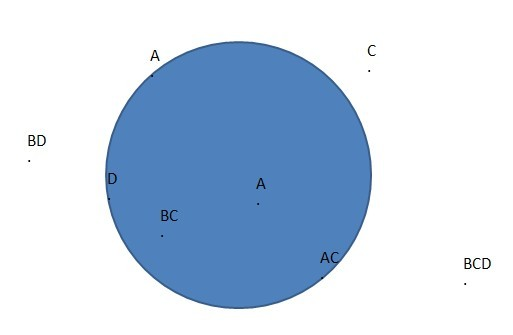
\includegraphics[width=2.5in]{figure/fig1}
\caption{An example of Smallest Enclosing Circle with query \{A,B,C,D\}.}
\end{center}
\end{figure}

\begin{theorem}\label{thm:lambda}
For a set of given points $P$ on the 2-dimensional plane,
the diameter of $P$ is $L$ and the diameter of
$P$'s smallest enclosing circle is $D$. If $|P|>1$ we have
the limition relationship: 
$ \frac{\sqrt{3}}{2} \cdot D\leq L \leq D$

\proof
Some proof here
\end{theorem}

The value of $\frac{\sqrt{3}}{2}$ will be mentional repeatedly,
so we use $\lambda$ to substitute this constant.
According to the above property, it's more clear if we
have the inequality changed into: $L \leq D \leq \frac{L}{\lambda}$.
This means if we find a circle with diameter $D$ and with
feasible objects inside we can make sure that
the result of diameter $L$ must be $[\lambda\cdot D,D]$
without any calculation. Namely, the upperbound and lowerbound
can be utilized to prune in the search space when even
the best lowerbound value can't lead to a better solution.

\begin{lemma}\label{lemma:monotone}
The value of diameter $D$ corresponding to the optimal solution
is monotonous. That is, if the circle covering the optimal solution
with a diameter $D$ we can always find a bigger circle with
diameter $D'(D' > D)$ that covers the optimal solution.

\proof
If set $S$ is the optimal solution of \textsf{TYPE2} problem,
we could find it's smallest enclosing circle $C$ with a diameter $D$.
The circle $C'$ with diameter $D'$ could fulfill the condition
if put outside the circle $C$.
\end{lemma}

An obvious opinion according to Lemma~\ref{lemma:monotone} is that
we devote to find a circle which both covering all the query keywords 
and with a diameter as small as possible. But according to
Theorem~\ref{thm:lambda} the reverse process is not absolutely
correct if we believe that the circle with the smallest diameter
will cover the optimal feasible solution. We will discuss this problem
and show how to fix it in the next part.

\subsection{Sweeping Circle} \label{subsec:type2:sweeping}
We just showed that a circle would help us to limit the objects
in some specific area. It's still challenging to find a concrete
position of the circle. We know that three points on the 2-dimensional plane
can determine a circle, but for the smallest enclosing circle problem we
have an analogous conclusion.
%

\begin{lemma}\label{lemma:boundary}
For a set of given points $P(|P|>1)$ on the 2-dimensional plane,
at least two points in $P$ are on the boundary of the smallest enclosing circle.

\proof
Let's utilize reduction to absurdity to prove. Suppose that only one point 
$P_i$ in $P$ is on the boundary of the circle $C$. If the diameter of $C$
is $D$, an $\epsilon$ exists such that a circle $C'$ with diameter $D-\epsilon$
and $C'$ is tangent to $C$ at point $P_i$. If any point is outside the
circle $C'$, we can decrease $\epsilon$ until all the points of $P$ inside
$C'$. Due to $D-\epsilon < D$, $C'$ is smaller than $C$ so $C$ is not
the smallest enclosing circle.
\end{lemma}

\begin{figure}\label{fig:4}
\begin{center}
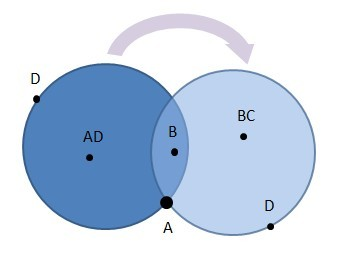
\includegraphics[width=2.5in]{figure/fig4}
\caption{Sweeping Circle Method Schematic Diagram}
\end{center}
\end{figure}

Now we can fix a point on the boundary of the circle based on Lemma~\ref{lemma:boundary}.
There is also an $O(nlogn)$ algorithm to calculate the diameter of given points 
which utilizes \textbf{Rotating Callipers in Convex Hull}. In the rotating callipers
algorithm, a convex hull is computed and two horizontal lines are defined
that enclose the points. Then rotate the lines together while proceeding along the
convex hull. In our problem we enumerate an object to be fixed and have the
diameter-determined circle rotated. If in a rotating angle all the objects inside
this circle cover all the query keywords, we can make sure that at least one feasible solution
exists among these objects. As we enumerate all the objects to be the fixed
one, even for the best solution one object must be on the boundary of the sweeping circle
according to Lemma~\ref{lemma:boundary}. Figure~\ref{fig:4} reflects the sweeping circle method
for query \{A,B,C,D\}.
Given the fixed object and a proper circle diameter $D$,
the best solution must be cover by the sweeping circle at a specific angle.
%

The sweeping circle strategy is based on an assumption that the circle diameter $D$
is given. Now we discuss how to determine the value of $D$ to get the
correct optimal results as well as avoiding useless enumeration with efficiency.
%

First, the correctness must be guaranteed. As we have introduced before, a smaller
diameter seems always better by intuition but whether the minimum diameter would 
not miss the optimal objects and guarantee the minimum value $L$?
%

\begin{example}\label{ex:counter}
Consider this situation as Figure~\ref{fig:2} and Figure~\ref{fig:3} shows:
Figure~\ref{fig:2} shows the furthest objects pair is exactly the diameter
of enclosing circle. Figure~\ref{fig:3} shows the three objects form an equilateral triangle.
Here we have $L_1 = \lambda\cdot D_1$ and $L_2 = D_2$ which reflects two extreme cases
of Theorem~\ref{thm:lambda} respectively. But if $L_1 < L_2$ and $D_1 > D_2$, we get
$\lambda\cdot D_1 < D_2 < D_1$ which is totally rational.
If we consider $D_2$ to be the lower bound to find the optimal solution,
we would miss $L_1$ which is a better result.
\end{example}
%

\begin{figure}\label{fig:2}
\begin{center}
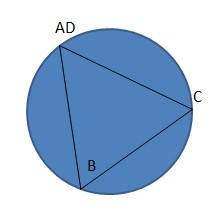
\includegraphics[width=1.5in]{figure/fig2}
\caption{Extreme case of diameter lower bound.}
\end{center}
\end{figure}

\begin{figure}\label{fig:3}
\begin{center}
\centering
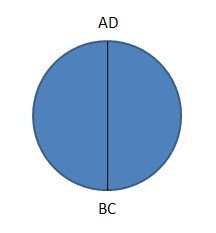
\includegraphics[width=1.5in]{figure/fig3}
\caption{Extreme case of diameter upper bound.}
\end{center}
\end{figure}

Example~\ref{ex:counter} shows a counter-example of considering the minimum
of diameter $D$ would cover the optiaml solution.

\begin{lemma}\label{lemma:enlarge}
Suppose $D$ to be the lower bound of diameter that could cover a feasible
set of objects. Sweeping circle with a diameter of $\frac{D}{\lambda}$ could
cover the optimal solution at some specific position.

\proof
Formally, let $L$ be the optimal distance of furthest pair objects,
and $L'$ be the second optimal one. We have $L \leq L'$.

According to Theorem~\ref{thm:lambda}, $L\leq D \leq \frac{L}{\lambda}$
where $D$ corresponds to the smallest enclosing circle.

Some proof here~
\end{lemma}

Second, we have known the lower bound value of diameter $D$ that covers at least
one feasible result could be utilized to ensure the correctness of
covering optimal result. Now we consider to compute it more efficiently.
The algorithm's idea is to perform a binary search to sovle this problem
in $O(logn)$ time cost. 
Based on Lemma~\ref{lemma:monotone}, the diameter $D$ is monotonous
that corresponds to the optimal solution. Actually, it's obvious to come
up with a same monotonous property to the feasible solution.
Formally, 
\begin{displaymath}
minD = \min{fesD_i}
\end{displaymath}
where $fesD_i$ is the minimum circle diameter to ensure a feasible solution
when we fix $object_i$ and perform the sweeping method. For a given diameter $D$,
we utilize sweeping circle method with a fixed $object_i$ by enumeration. If $D<minD$
we can't find any feasible solution, then we'll try a larger diameter.

The pesudocodo is given in Algorithm~\ref{alg:binarysearch}. In lines 1-2,
we set the initial interval to be $(low, high)$ here $\infty$ can be set as a very
large value to ensure that the initial interval would not miss the optimal solution.
In line 3-13, we perform a binary search framework iteratively approach the $minD$.
We check the median value $D$ of current seach interval. By enumerating all the objects (line 6)
and fixing this object as pivot we invoke the $circle\_scan()$ function
to inspect whether a feasible solution exists with diameter $D$.
If any feasible position is found we can ensure that $minD < D$, so in next iteration
only consider the left interval $(low,D)$. Conversely, the right interval $(D,high)$
needs to be searched. We set an $eps$ to restraint the binary search steps where
$eps$ is a very small value. So the stoping criteria for the binary search is the length
of current searching interval exceed $eps$ (line 3). 

When the $minD$ has been determined, we enlarge the value of $D$ by dividing $\lambda$
(line 14) according to Lemma~\ref{lemma:enlarge} to ensure the correctness for the optimal
solution. Then for each pivoit object we invoke $circle\_scan()$ to find specific positions and perform
the exhuastive search to compute the concrete result, because the circle limitation strategy
only points out the potential area but different combinations of objects may lead to
different results. Actually, this is the original \textsf{TYPE2} problem we want to sovle, but
the number of objects has been greatly reduced.

%\textbf{Add an example here}

In this binary seach framework
we invoke function $circle\_scan()$ twice with the third parameter different .
Both of them perform the circle sweeping with an object as the pivot and rotate the
circle to find one or more specific angle where all the objects inside the circle would
cover all the keywords. For the first invoking we don't need to
know the concrete combination, because based on Theorem~\ref{thm:lambda} we have
$L$ ranges in $[\lambda\cdot D, D]$.
But for the second invoking, after a potential area has been found
an exhausted search is invoked to compute exact result in this circle area.

\begin{algorithm}[!ht]\small\label{alg:binarysearch}
\caption{ \bf {Framework of Binary Search} (objects,eps)}

$low \gets 0$\;
$high \gets \infty$\;
\While{$high - low > eps$}{
	$D \gets (high + low)/2$\;
	$is\_any\_objects\_possible \gets false$\;
	\For{each object in objects}{
		\If{$circle\_scan(object,D,false)$}{
			$is\_any\_objects\_possible \gets true$\;
			break\;
		}
	}

	\eIf{$is\_all\_objects\_possible$}{
		$high \gets D$\;
	}{
		$low \gets D$\;
	}
}
$D \gets D/\lambda$\;
\For{each object in objects}{
	$circle\_scan(object,D,true)$\;
}
\Return $D$\;\vspace{-1ex}

\end{algorithm}

Let $object_i$ to be the fixed pivot and $D$ to be the sweeping circle diameter.
If all other objects that in the circle with $2D$ as diameter and $object_i$ as
the center can't cover all the query keywords, any feasible solution can't
be found. It's a obvious pruning that showed in Figure~\ref{fig:5} where the
bigger circle with $2D$ as diameter is the total sweeping area.

\begin{figure}\label{fig:5}
\begin{center}
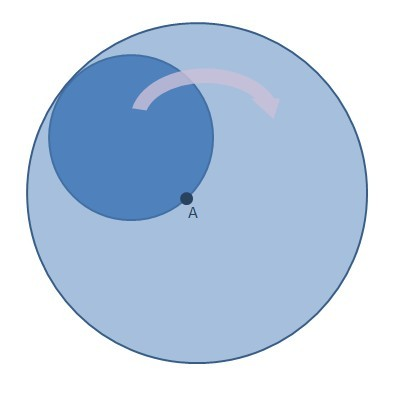
\includegraphics[width=1.5in]{figure/fig5}
\caption{Sweeping Area}
\end{center}
\end{figure}

Then we introduce how to perform the function $circle\_scan()$, that is, the circle
sweeping process. For each object in the scan area, if we sweep the circle by $360$
degree it will be covered by the circle once. Because each object is scaned
ouside-in or inside-out by the circle exactly once. The shape of the circle is
given and one pivot on the boundary is fixed, so for each $object_i$ it's possible
to compute the specific angle $angle\_out_i$ when be scaned outside-in and the
angle $angle\_in_i$ when be scaned inside-out. Actually, clockwise or
counter-clockwise sweep makes no difference, so we might as well take the clockwise.
For each object we have computered the two angles respectively, then sort all these angles. 
We use minimum increment method to sweep the cirle, that is, for the current sweeping
angle  we choose whether to sweep in a new object or sweep out an old
object that coverd by current circle.

\begin{figure}\label{fig:7}
\begin{center}
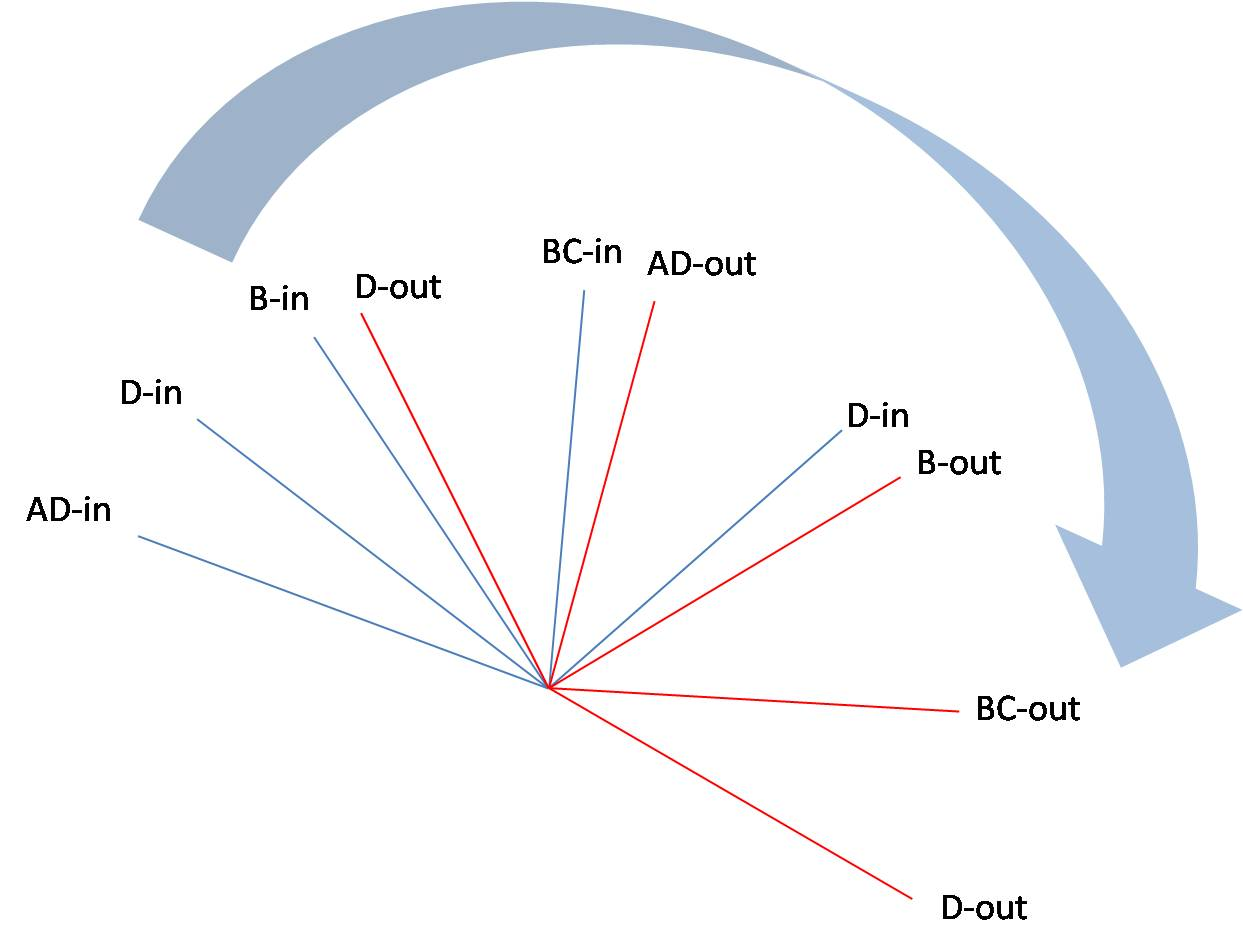
\includegraphics[width=2.5in]{figure/fig7}
\caption{Circle Scan with Minimum Incrememt}
\end{center}
\end{figure}

Figure~\ref{fig:7} shows the minimum incrememt sweeping of the case in Figure~\ref{fig:4}.
We map the position where an object swept out of the circle and the position where
an object swept into the circle to polar angles of red and blue color respectively.
In each step we only move the polar angle to the next position with minimum increment,
either cover a new object into the circle or pop-up the last object out of the circle.
The polar angles need to be sorted initially and be scanned one by one. 
Sorting these angles costs $O(nlogn)$ and the $angle\_in$ and $angle\_out$ are exactly
scanned once during the sweeping which costs $O(n)$, so the time complexity for a circle sweeping is $O(nlogn)$.

The \textsf{TYPE2} problem is made up of two parts, and we have disregarded the
first part. When consider the distance between the furthest object and the query location,
we need to adjust the algorithm to fit the differences. The furthest object to the
query actually is on the boundary of the circle, so when we enumerate which object
to be the rotating pivot we can treat this object to be the furthest object. So all
the other objects swept should be nearer than the pivot. When we perform the binary search
we also consider the distance between the pivot and the query location.

\begin{algorithm}[!ht]\small\label{alg:binarysearch2}
\caption{ \bf {Framework of Binary Search for TYPE2 problem} (objects,q,eps)}

$low \gets 0$\;
$high \gets \infty$\;
\While{$high - low > eps$}{
	$totcost \gets (high + low)/2$\;
	$is\_any\_objects\_possible \gets false$\;
	\For{each object in objects}{
		$D \gets totcost-Dist(object,q)$\;
		\If{$circle\_scan(object,D,false)$}{
			$is\_any\_objects\_possible \gets true$\;
			break\;
		}
	}

	\eIf{$is\_all\_objects\_possible$}{
		$high \gets totcost$\;
	}{
		$low \gets totcost$\;
	}
}
\For{each object in objects}{
	$D \gets totcost-Dist(object,q)$\;
	$circle\_scan(object,D/\lambda,true)$\;
}
\Return $totcost$\;\vspace{-1ex}

\end{algorithm}

The presudocode is described in Algorithm~\ref{alg:binarysearch2}. One of the differences
is we utilize binary search for $totcost$ instead of $D$ which is the sum of $D$ and $Dist(object,q)$ (lines 7-8).
Another difference is when the lower bound of $totcost$ has been found we enlarge the diameter by dividing $\lambda$ (line 17)
but not the $totcost$.

\subsection{Enumerate the best group containing an object}\label{subsec:type2:search}
When we have found several circle positions that covers all the query keywords during the sweeping,
an exhuastive search \textsf{getCandidiateSet()} is invoked to compute the combination of objects. 
Unfortunately, if the number of candidiate objects 
is too large the time cost increases exponentially. To facilitate more efficient checking,
we use some pruning strategies based on textual and geometric properties. 
Suppose $curCost$ to be the optimal result for \textsf{MAX+MAX SKG} problem,
the value of $curCost$ is updated during the exhaustive search. 

A reasonable search approach is to append a new object to the current selected object set and
perform the search iteratively.
This new object must cover a new keyword which has not been covered by the selected set.
The deepest level of this depth-first-search is at most the number of query keywords because each object
contains at least one new keyword.
Let $selectedCost$ be the furthest distance of any selected object pair and
$furthestDist$ to be the distance between the pivot and query location, the goal is to
make $selectedCost+furthestDist<curCost$ and update $curCost$ while covering all query keywords.
%

According to the cost function definition, the first \textsf{MAX} is related to only
the furthest object to the query. Based on this observation, we first choose an object to be
the furthest object, so the search space is greatly reduced. Formally, let $o_f$ to be the furthest
object we enumerated, an object $o$ should not be taken into consideration 
iff $\textsf{Dist}(o,query)>\textsf{Dist}(o_f,query)$.

\begin{algorithm}[!ht]\small\label{alg:search}
\caption{ \bf {enumerateBestGroup} (objectSet, pivot, diameter)}

sort $objectSet\ by\ \textsf{Dist}(query,*)$\;
$candidateSet\gets \emptyset$\;
$keywords\gets pivot.\psi$\;

\For{each object in objectSet}{
	$selectedSet\gets \{pivot, object\}$\;
	$candidateSet\gets candidateSet + object$\;
	$pairDist\gets \textsf{Dist}(pivot, object)$\;
	$furthestDist\gets \textsf{Dist}(query, object)$\;
	$keywords\gets keywords\cup object.\psi$\;
	\If{$keywords=query.\psi$}{
		$localSearch(selectedSet, candidateSet, pairDist,$\
		$furthestDist, pivot.\psi\cup object.\psi, 0)$\;
	}
}

\end{algorithm}
The presudocode is described in Algorithm~\ref{alg:search}.
The first step is to determine the furthest object. We sort all the objects
according to their ascending distance to the query location (Line 1).
In line 6, each object is added to the candidateSet one by one to make sure that
the last added object must be the furthest to the query location.
The selectedSet initially contains only $pivot$ and the furthest object we choosed,
so the distance and textual value are initialized respectively (Line 7-9).
Finally, when the $candiadateSet$ could cover all query keywords
we call the function $localSearch()$ to search the optimal solution
iteratively(Line 10-11).

\begin{algorithm}[!ht]\small\label{alg:localSearch}
\caption{\bf{localSearch} (selectedSet, candiadateSet, pairDist, furthestDist, keywords, startId)}
\If{$keywords = query.\psi$}{
	\If{$furthestDist + pairDist < curCost$}{
		$curCost\gets furthestDist + pairDist$\;
		$curGroup\gets selectedSet$\;
	}
	\Return $curCost$\;
}
\If{$furthest+pairDist > curCost$}{
	\Return $curCost$\;
}
$nextSet\gets \emptyset$\;
$leftKeyowrds\gets \emptyset$\;
\For{each candiadate in candiadateSet}{
	\If{$ (query.\psi - keywords) \cap candiadate.\psi = \emptyset $}{
		\textbf{continue}\;
	}
	\If{$candiadate.Id<startId$}{
		\textbf{continue}\;
	}
	$candiadate.dist\gets 0$\;
	\For{each selectedObject in selectedSet}{
		$candiadate.dist=max(candiadate.dist, \textsf{Dist}(selectedObject, candiadate))$\;
	}
	\If{$candiadate.dist+furthestDist>curCost$}{
		\textbf{continue}\;
	}
	$nextSet\gets nextSet+candiadate$\;
	$leftKeywords\gets leftKeywords+candiadate.\psi$\;
}

\If{$leftKeywords\cup keywords != query.\psi$}{
	\Return $curCost$\;
}

\For{each object in nextSet}{
	$selectedSet\gets selectedSet\cup object$\;
	$localSearch(selectedSet, nextSet, max(pairDist,candiadate.dist),furthestDist, keywords\cup object.\psi, object.Id)$\;
	$selectedSet\gets selectedSet - object$\;
}
\end{algorithm}
\end{document}
